In this section we derive the conservation equations using a two-fluid formulation.
While the derivation of this formulation is available in various studies such as those by \citet{kataoka1986local,lhuillier2010multiphase,ishii2010thermo,morel2015mathematical,bothe2022sharp} our approach here enables us to introduce specific notations and key results that will prove useful for later discussions. %
\begin{figure}[h!]
    \centering
    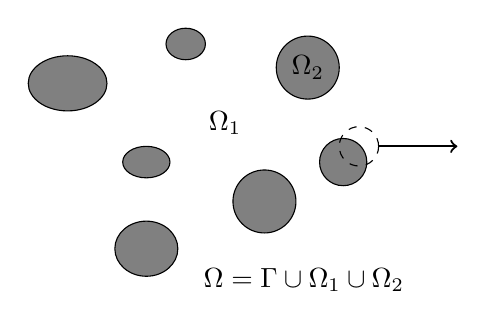
\begin{tikzpicture}
        \foreach \x/\y/\ra/\r in {
        1/3/0.2/0.25,
        2.55/2.7/0.4/0.4,
        0.5/0.4/0.35/0.4,
        2/1/0.4/0.4,
        3/1.5/0.3/0.3,
        0.5/1.5/0.2/0.3,
        -0.5/2.5/0.35/0.5}{
            \draw[fill=gray](\x,\y) ellipse(\r cm and \ra cm);
        }
        \draw[dashed](3.2,1.7)circle(0.25);
        % \draw[thick,->](3.2,1.7)++(0.1767,0.1767)--++(0.4,0.4)--++(1,0);
        \draw[thick,->](3.2,1.7)++(0.25,0)--++(1,0);
        \draw(2.55,2.7)node{$\Omega_2$};
        \draw(1.5,2)node{$\Omega_1$};
        \draw(2.5,0)node{$\Omega = \Gamma \cup \Omega_1 \cup \Omega_2$};
        % \draw(2.5,-1)node{$\Gamma = \sum_\alpha \Gamma_\alpha$};
        % \draw(2.5,-0.5)node{$\Omega_2 = \sum_\alpha \Omega_\alpha$};
    \end{tikzpicture}
    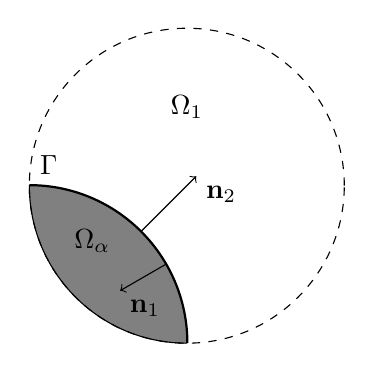
\begin{tikzpicture}%[scale = 0.9]
        \draw[very thick](0:2)arc(0:90:2)node[above right]{$\Gamma$};
        \draw[fill=gray](0:2)arc(0:90:2)arc(180:270:2);
        \draw[dashed](2,2)circle(2);
        \draw[->](1.42,1.42)--++(0.7,0.7)node[below right]{$\textbf{n}_2$};
        \draw[->](1.73,1)--++(-0.577,-0.333)node[below right]{$\textbf{n}_1$};
        \draw(2,3)node{$\Omega_1$};
        \draw(0.8,1.3)node{$\Omega_\alpha$};
    \end{tikzpicture}
    \caption{Topology of dispersed two-phase flows.}%Domain definitions and scheme of the topology of dispersed two-phase flows.}
    \label{fig:Scheme}
\end{figure}

We consider a system consisting of two phases, separated by a sharp interface $\Gamma(t,\FF)$ where $\FF$ is a given flow configuration which evolves over time $t$. 
Each phase subdomain is denoted as $\Omega_1(t,\FF)$ and $\Omega_2(t,\FF)$, representing the continuous phase (1) and the dispersed phase (2) respectively (refer to Figure \ref{fig:Scheme}).
The entire domain, denoted as $\Omega$, is defined as the union of $\Omega_1$, $\Omega_2$, and $\Gamma$.
To track the position of the phase indexed $k$ and the interfaces, we introduce the phase indicator function $\chi _k$ defined as
\begin{align}
    \chi_k(\textbf{x},t,\FF) =  \left\{
      \begin{tabular}{cc}
        $1 \;\text{if} \;\textbf{x} \in \Omega_k(t,\FF)$\\
        $0 \;\text{if} \;\textbf{x} \notin \Omega_k(t,\FF)$
      \end{tabular}
      \right.
      \text{for $k = 1,2$}.
      \label{eq:PIF}
\end{align}

\subsection{Topological equations}
Using the distribution formalism, one may show that $\chi_k(\textbf{x},t,\FF)$ obeys the following relations \citep{drew1983mathematical,orlando2023evolution}. 
\begin{align}
    \pddt \chi_k
    + \textbf{u}_I^0 \cdot \grad \chi_k
    &= 0,
    \label{eq:dt_chi_k}\\
    \label{eq:grad_chi_k}
    \grad \chi_k
    &= - \delta_I \textbf{n}_k, 
\end{align}
where $u^0_I(\textbf{x},t,\FF)$ is the velocity of the interface and $\delta_I(\textbf{x},t,\FF)$ is the Dirac function localized on the interface.
All along this work we employ the subscript $_I$ to indicate any quantity inherently defined on the interface such as its local velocity $\textbf{u}_I^0(\textbf{x},t,\FF)$. 
Additionally, we use the superscript $^0$ to indicate that the variable is defied at the local or microscopic scale, in opposition to the averaged or macroscopic quantities that will be presented latter. 
Thus, it must be understood that all local quantities denoted by a $^0$, are function of the flow configuration $\FF$, the position vector $\textbf{x}$, and the time $t$. 
To enhance clarity, we will omit the arguments from $\chi_k(\textbf{x},t,\FF)$, $\delta_I(\textbf{x},t,\FF)$ and any local function denoted by a $^0$ in the subsequent sections.
Then, to describe the evolution of $\delta_I$ we take the gradient for \ref{eq:dt_chi_k} and the gradient of \ref{eq:grad_chi_k} which yields two equations of the interface indicator function \citep{marle1982macroscopic,morel2007surface,orlando2023evolution},
\begin{align}
    \pddt \delta_I
    + \div [\delta_I (\textbf{u}_I^0\cdot \textbf{n}) \textbf{n}]
    &= \delta_I (\textbf{u}_I^0 \cdot \textbf{n})(\div\textbf{n})
    \label{eq:dt_delta_I}\\
    \grad\delta_I 
    &= \textbf{n} \cdot \grad (\textbf{n} \delta_I),
    \label{eq:grad_delta_I}
\end{align}
Furthermore, notice that we did not specify the index of the normal $\textbf{n}$ in \ref{eq:dt_delta_I} and \ref{eq:grad_delta_I}. 
This is because the normal vector appears twice in each terms of these equations, making the expression independent of the sign of $\textbf{n}$.
Additionally, only the normal components of the surface velocity play a role in \ref{eq:dt_delta_I}. 
And $\div \textbf{n}$ represents the curvature of the interfaces. 


\ref{eq:dt_chi_k}, \ref{eq:dt_delta_I}, \ref{eq:grad_delta_I} and \ref{eq:grad_chi_k} are commonly referred to as the topological equations. 
It describes the evolution in space and time of the topology of the flow interfaces.

\subsection{Local conservation equations}
\label{sec:local_eq}
Let now introduce the local conservation laws that govern the fluid inside bulk phases and the interfaces. 

\subsubsection{Inside the volumes}

Within phase $k$, we note $\rho_k^0$ the density, $\textbf{u}_k^0$ the local velocity and $E_k^0$ the local total energy per units of mass.
All over the domain $\Omega_k$ the mass, momentum and total energy obey these conservation laws :
\begin{align}
    \label{eq:dt_rho}
    \pddt \rho_k^0  
    + \div (
        \rho_k^0\textbf{u}_k^0
    )
    &= 
    0\\
    \label{eq:dt_rhou_k}
    \pddt (\rho_k^0\textbf{u}_k^0)  
    + \div (
        \rho_k^0\textbf{u}_k^0\textbf{u}_k^0
        - \bm{\sigma}_k^0 
    )
    &= 
    \rho_k^0 \textbf{g}\\
    \label{eq:dt_rhoE_k}
    \pddt (\rho_k^0E_k^0)  
    + \div (
        \rho_k^0E_k^0\textbf{u}_k^0
        + \textbf{q}_k^0
        - \textbf{u}_k^0 \cdot \bm{\sigma}_k^0 
        )
    &= 
    \textbf{u}_k^0 \cdot \textbf{g}  \rho_k^0
\end{align} 
All along this work the continuous phase will be considered as Newtonian fluid thus, $\bm{\sigma}_1^0 = - p_1^0 \bm\delta + \bm{\tau}_1^0$ where $\bm{\tau}_1^0 = \mu_1[\grad \textbf{u}_1^0+(\grad \textbf{u}_1^0)^\dagger]$ is the Newtonian stress tensor with $p_1 ^0$ the local pressure. 
The vector $\textbf{q}_k^0$ represent the thermal energy flux and is often model with a Fourier law : $\textbf{q}_k^0 = -\lambda \grad T_k^0$ where $T_k^0$ is the temperature. 
$\textbf{g}$ is the acceleration of gravity which will be the only body force in the present problem. 

The total energy is decomposed in the usual way, i.e. $E_k^0 = e_k^0 + (u_k^0)^2/2$ where  $e_k^0$ is the internal energy per unit of mass which represent the molecular agitation and $(u_k^0)^2/2$ is the kinetic energy per unit of mass.
This decomposition and the previous set of equations lead us to two independent equations for $e_k^0$ and $(u_k^0)^2/2$, namely,
\begin{align}
    \label{eq:dt_rhou_k2}
    \pddt [\rho_k^0(u_k^0)^2]  
    + \div [\rho_k^0(u_k^0)^2\textbf{u}_k^0/2 - \textbf{u}_k^0 \cdot \bm{\sigma}_k^0]
    &=
    \rho_k^0\textbf{u}_2^0 \cdot \textbf{g}  
    -  \bm{\sigma}_k^0 : \grad \textbf{u}_k^0,
    \\
    \label{eq:dt_rhoe_k}
    \pddt (\rho_k^0e_k^0)  
    + \div (
        \rho_k^0e_k^0\textbf{u}_k^0
        + \textbf{q}_k^0
        )
    &= 
    \bm{\sigma}_k^0 : \grad \textbf{u}_k^0. 
\end{align} 
We can observe that the viscous dissipation term, $\bm{\sigma}_k^0 : \grad \textbf{u}_k^0$,  appears with opposite sign in both of the above equations.
This indicates that the amount of energy transformed from kinetic to internal energy is given by $\bm{\sigma}_k^0 : \grad \textbf{u}_k^0$, which is the viscous dissipation. 
By the use of constitutive laws one can show that the internal energy equation can be re-written into an equation for the local temperature $T_k^0$ \citep{ishii2010thermo}.
% In this study, we concentrate on the mechanical energy equations and do not consider thermodynamic aspects.  
% Thus, in the following we provide the internal energy equaiton 

\subsubsection{On interfaces}

On the interface $\Gamma$ the conservation laws take the form of $2D$ conservation laws due to the topology of the interface. 
They are often viewed as \textit{jump conditions} which make the link between the conservation equations in both phases. 
The interface mass and momentum conservation equations are well established.
However, the energy jump condition is less employed, and therefore needs some clarification.
In the most general case the mass, momentum and energy surface equations can be written as \citep{ishii2010thermo,morel2015mathematical,bothe2022sharp}, 
\begin{align}
    \label{eq:dt_rhoI}
    \pddt \rho_I^0
    % + \rho_I^0 (\textbf{u}_I^0 \cdot \textbf{n})(\div \textbf{n})
    + \divI (\rho_I^0\textbf{u}_{I}^0)
    &= 
    -\Jump{
        \rho_k^0 (\textbf{u}_I - \textbf{u}_k)
    }
    \\
    \label{eq:dt_rhoIu_I}
    \pddt (\rho_I^0\textbf{u}_I^0)  
    % + \rho_I^0 \textbf{u}_I^0 (\textbf{u}_I^0 \cdot \textbf{n})(\div \textbf{n})
    + \divI (
    \rho_I^0\textbf{u}_I^0\textbf{u}_{I}^0
    - \bm{\sigma}_{I||}^0)
    &= 
    \rho_I^0 \textbf{g}
    - \Jump{
        \rho_k^0 \textbf{u}_k (\textbf{u}_I - \textbf{u}_k)
        + \bm\sigma^0_k
    }
    \\
    \label{eq:dt_rhoIE_I}
    \pddt (\rho_I^0E_I^0)  
    % + \rho_I^0E_I^0  (\textbf{u}_I \cdot \textbf{n})(\div \textbf{n})
    + \divI (
        \rho_I^0 E_I^0\textbf{u}_{I}^0
        - \textbf{u}_I^0 \cdot \bm{\sigma}_I^0 
        + \textbf{q}_{I||}^0
        )
    &= 
    \textbf{u}_I^0 \cdot \textbf{g}  \rho_I^0
    - \Jump{\textbf{u}_k^0 \cdot \bm{\sigma}_k^0 - \textbf{q}_k^0
    + \rho_k^0 E_k (\textbf{u}_I - \textbf{u}_k)
    }
\end{align} 
where, $\rho_I^0$ is the mean density of the interface per unit of surface area,  
$\textbf{u}_I^0$ is the local velocity of the interface, $E_I^0 = e_I^0 + \frac{1}{2}(u_I^0)^2$ is the total energy with $e_I^0$ the internal energy, $\bm{\sigma}_I^0$ is the momentum diffusive flux through the surface and $\textbf{q}_I^0$ is the heat flux on the surface.  
We introduced the surface divergence operator defined as $\divI ()= (\bm\delta-\textbf{nn})\cdot \div ()$, which correspond to the divergence operator projected on $\Gamma$. 
Throughout this work we use the subscript  $_{||}$ to indicate the projection of a quantity onto the plane tangential to the surface $\Gamma$. 
Specifically, for an arbitrary quantity $\textbf{f}$ defined on $\Gamma$, we denote its tangential projection as $\textbf{f}_{||} = (\bm\delta-\textbf{nn})\cdot \textbf{f}$. 
Notice that the diffusive flux $\bm{\sigma}_{I||}^0$ appear as a quantity projected on the surface tangential plane.
Indeed, it can be shown that only the tangential parts of the diffusive flux plays a role in the surface momentum balance equations \citep{slattery2007interfacial,bothe2022sharp}.
We also introduced the notation $\Jump{\ldots}$, which is defined as $\Jump{\ldots} = \sum_{k=1}^2 [\ldots] \cdot \textbf{n}_k$.
Where $\textbf{n}_k$ is the outward normal vector associated with the domain $\Omega_k$ (see \ref{fig:Scheme}).
Therefore, the terms on the right-hands side of \ref{eq:dt_rho_I}, \ref{eq:dt_rho_Iu_I} and \ref{eq:dt_rho_IE_I} represent the source terms due to the discontinuity of the bulk properties from each side of the interface $\Gamma$ and the phase transfer terms. 
For further insights into the modeling of sharp interface thermodynamics, a comprehensive review may be found in \cite{bothe2022sharp}. 

The formulation given by \ref{eq:dt_rho_I},\ref{eq:dt_rhoIu_I}and \ref{eq:dt_rhoI} remains quite general and needs some further simplifications. 
Therefore, we consider that :
(1) The mass, momentum and kinetic energy per unit of surface can be neglected, i.e. $\textbf{u}_I^0\rho_I = 0 $ and $(u_I^0)^2\rho_I = 0$. 
Implying that the surface source terms are also neglected, here $\rho_I \textbf{u}_I^0\cdot \textbf{g} = 0$; 
(2) No mass transfer is allowed at the interface, together with the previous assumption this implies that $\textbf{u}_k^0 = \textbf{u}_I^0$ for $k = 1,2$. 
(3) All molecular diffusion fluxes can be neglected, i.e. the viscous stress at the interfaces as well as the surface heat flux can be neglected.
Therefore, the surface stress tensor is assumed isotropic on the surface, and is written $\bm{\sigma}_I^0  = \gamma (\bm\delta - \textbf{nn}) = \gamma \bm\delta_{||}$ where $\gamma$ is the constant surface tension coefficient.
Under this hypothesis the internal energy and the surface tension coefficient are related through $\phi_I^0 e_I^0 = \gamma$ \cite{ishii2010thermo};
% When using a constant surface tension coefficient the interfacial mass, momentum and total energy balance equations reduce to the expressions,
Under these restrictive assumptions we obtain the following set of governing equations for the interfaces,
\begin{align}
    \label{eq:dt_rho_I}
    \textbf{u}_k = \textbf{u}_I^0, \\
    \Jump{\bm{\sigma}_k^0} 
    &=
    \divI\bm\sigma^0_{I||}
    =
    -\gamma\textbf{n}(\div \textbf{n}),
    \label{eq:surface_tension}\\
    \label{eq:dt_rhoI_EI}
    \Jump{\textbf{u}_k^0 \cdot \bm{\sigma}_k^0 - \textbf{q}_k^0}
    &=
    -\gamma\textbf{n}\cdot \textbf{u}_{I}^0(\div \textbf{n})
\end{align}
respectively. 
% The jump condition for the total energy can be separated into an expression for the kinetic and internal energy. 
By taking the dot product of \ref{eq:surface_tension} with $\textbf{u}_I^0$ and subtracting this first expression to \ref{eq:dt_rhoI_EI}, gives us
\begin{align}
    \label{eq:dt_rhoI_uI3}
    \Jump{\textbf{u}_k^0 \cdot \bm{\sigma}_k^0}
    &=
    -\gamma\textbf{n}\cdot \textbf{u}_{I}^0(\div \textbf{n})\\
    \label{eq:dt_rhoIe_I}
    \Jump{ \textbf{q}_k^0}
    &= 
     0
\end{align}
which are the interface kinetic energy and the internal interface energy jump condition, respectively. 
As witnesses by \ref{eq:dt_rhoI_uI3} the discontinuity of mechanical energy through the surface is equivalent to the work of the tension forces. 

\subsubsection{Generic formulation}

For ease of understanding, we now introduce generic conservation laws in the volumes and on the interfaces. 
Let $f_k^0$ denote a volumetric quantity of arbitrary tensorial order defined in $\Omega_k$.
Likewise, let $f_I^0(\textbf{x}_I,I)$ represent an arbitrary surface property defined on $\Gamma$.
Using the strategy outlined in \citep{ishii2010thermo,bothe2022sharp}, the local conservation equations for $f_k^0$ and $f_I^0$ yield,  
\begin{align}
    \label{eq:dt_f_k}
    \pddt f_k^0
    +\div \left(
        f_k^0\textbf{u}_k^0
        - \mathbf{\Phi}_k^0
        \right)
    &= 
    s_k^0
    & \text{ in } \Omega_k,&\\
    \pddt f_I^0 
    + f_I^0 (\textbf{u}_I \cdot \textbf{n})(\div \textbf{n})
    +\divI
    (f_I^0 \textbf{u}_{I||}^0
        - \mathbf{\Phi}_{I||}^0 )
    &= 
    s_I^0
    - \Jump{
       f_k (\textbf{u}_I^0 - \textbf{u}_k^0)
       + \mathbf{\Phi}_k^0
    } 
    & \text{ on } \Gamma,&
    \label{eq:dt_f_I}
\end{align}
respectively.
The tensors $\mathbf{\Phi}_k^0(f_k^0)$ and $\mathbf{\Phi}_{I||}^0(f_I^0)$ represent the non-convective fluxes corresponding to the quantities $f_k^0$ and $f_I^0$, respectively. 
Notice that $\mathbf{\Phi}_{I||}^0$ also carries the $_{||}$ subscript which implies that only the tangential component of this tensor plays a role in the surface balance equation. 
Similarly, $s_k^0(f_k^0)$ and $s_I^0(f_I^0)$ represent the source terms of $f_k^0$ and $f_I^0$, respectively.
Notice, that in \ref{eq:dt_f_I} we kept the mass transfer term $f_k (\textbf{u}_I^0 - \textbf{u}_k^0)$ for purpose of generality. 
The second term on the right-hand side of \ref{eq:dt_f_I} represents the fluxes due to the deformation of the interfaces, and the third term represents the 2D fluxes on the surface. 
For practical uses, note that the advecting term in \ref{eq:dt_f_I} can be written in the more compact form $f_I^0 (\textbf{u}_I \cdot \textbf{n})(\div \textbf{n})
+\divI(f_I^0 \textbf{u}_{I||}^0) = \divI(f_I^0 \textbf{u}_I^0)$ by noticing that $\textbf{n}\cdot\gradI(\ldots) = 0$ and $\divI\textbf{n} = \div\textbf{n}$ \citep{nadim1996concise}.
It is important to note that \ref{eq:dt_f_k} and \ref{eq:dt_f_I} are defined uniquely int the domains $\Omega_k$ and $\Gamma$, respectively.
% Consequently, these equations are referred to as local conservation equations. 


\subsection{The two-fluid formulation}
The presence function $\chi_k$, and the Dirac delta function $\delta_I$, allow the extension of \ref{eq:dt_f_k} and \ref{eq:dt_f_I} to the entire flow domain $\Omega$. 
This extension is achieved by employing the methodology introduced by \citet{drew1983mathematical} and \citet{kataoka1986local} for the conseriving laws inside the volume (\ref{eq:dt_f_k}).
For any local quantities $f_k^0$ defined in $\Omega_k$, we assign the field $\chi_k f_k^0$, which is defined over the entire domain $\Omega$. The two-fluid formulation may be obtained by multiplying \ref{eq:dt_f_k} by $\chi_k$. 
Using \ref{eq:dt_chi_k} and \ref{eq:grad_chi_k} we obtain
\begin{equation}
    \pddt (\chi_k f_k^0)
    + \div (
        \chi_k f_k^0 \textbf{u}_k^0
        - \chi_k \mathbf{\Phi}_k^0 
        )
    = 
    \chi_k s_k^0
    + \delta_I\left[
        f_k^0
        \left(
            \textbf{u}_I^0
            - \textbf{u}_k^0
        \right)
        + \mathbf{\Phi}_k^0
    \right]
    \cdot \textbf{n}_k.
    \label{eq:dt_chi_k_f_k}
\end{equation}
Likewise, for any surface property $f_I^0$ defined on $\Gamma$, we assign the field $\delta_I f_I^0$, which is also defined all over $\Omega$. 
% Following the approach outlined \citet[Appendix 2]{marle1982macroscopic} we can generalize \ref{eq:dt_f_I} to the 3D space. 
Then, multiplying \ref{eq:dt_f_I} by $\delta_I$ and making use of the topological equations \ref{eq:dt_delta_I} and \ref{eq:grad_delta_I} gives,
\begin{equation}
    \pddt (\delta_If_I^0)  
    + \div (
        \delta_I f_I^0 \textbf{u}_I^0
        - \delta_I \mathbf{\Phi}_{I||}^0 
        )
    = 
    \delta_Is_I^0
    - \delta_I\Jump{
    f_k^0 (\textbf{u}_I^0 - \textbf{u}_k^0)
    + \mathbf{\Phi}_k^0} 
    \label{eq:dt_delta_I_f_I}
\end{equation}
which correspond to the conservation equation for $\delta_If_I^0$.
As the derivation of \ref{eq:dt_delta_I_f_I} is not straightforward we provide intermediate steps in \ref{ap:interface_proof}. 
The last terms on the right hands side of \ref{eq:dt_chi_k_f_k} represent the phase transfer of $f_k$ across the interfaces and the source due to the discontinuity of the non-convective fluxes across phases.
Note that these terms act as sinks in the right-hand side of \ref{eq:dt_delta_I_f_I}. 
The set of equations formed by \ref{eq:dt_chi_k_f_k} for $k =1,2$ to which we add the surface transport equation or \textit{jump condition} (\ref{eq:dt_delta_I_f_I}) is commonly known as the \textit{two-fluid} formulation of multiphase flows \citep{morel2015mathematical,tryggvason2011direct,drew1983mathematical,kataoka1986local}. 

% \tb{this formulation is useful for the bulk stress}
In this work, we prefer to think of those equations as a set of three equations formed by \ref{eq:dt_chi_k_f_k} for $k=1,2$ and \ref{eq:dt_delta_I_f_I}. 
We define the \textit{bulk} property $\textbf{f}$ as $\textbf{f}^0 = \sum_k \chi_k \textbf{f}_k^0 + \delta_I \textbf{f}_I^0$ where $\textbf{f}^0$ represents any property of the flow of arbitrary tensorial order at the local scale.
Then by summing \ref{eq:dt_chi_k_f_k} for $k=1,2$ and \ref{eq:dt_delta_I_f_I}, one obtain the \textit{single-fluid} formulation conservation equation, namely,
\begin{equation}
   \pddt f^0
   + \div (
       f^0 \textbf{u}^0
       -  \mathbf{\Phi}^0 
    )
   = s^0. 
   \label{eq:dt_f}
\end{equation}
It should be noted that in the literature we rather define the \textit{bulk} quantities as $f^0 = \sum_k \chi_k f_k^0$, while the interfacial component is treated as a source term in \ref{eq:dt_f} \citep{morel2015mathematical,tryggvason2011direct,drew1983mathematical}. 
Nevertheless, we want to point out here that with this definition we recover a classic transport equation for the bulk quantity $f^0$ which makes the whole system of equation consistent.



